\section{Anhang}
\subsection{Abbildungen}
\subsubsection{Lichtwellen}
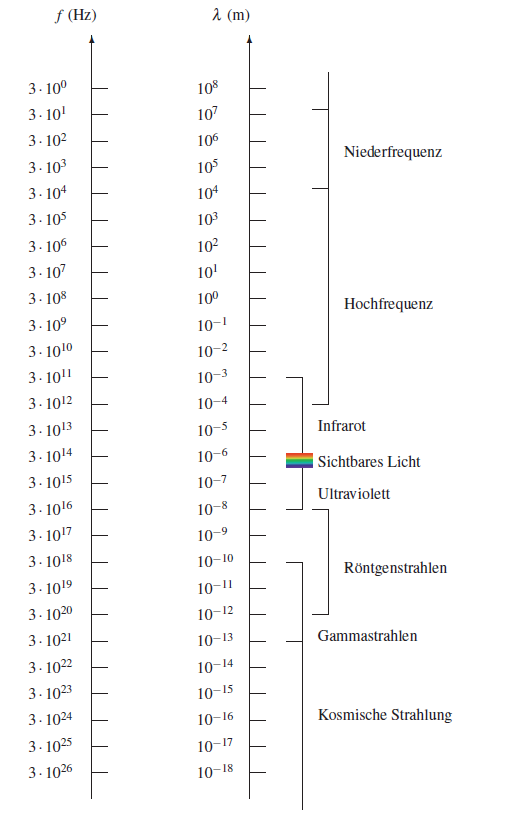
\includegraphics[height=7cm,center,keepaspectratio=true]{Images/lichtwellen.png}

\subsection{Tabellen}

\begin{center}
	\refkuchling{627f.}, Tabelle 9
	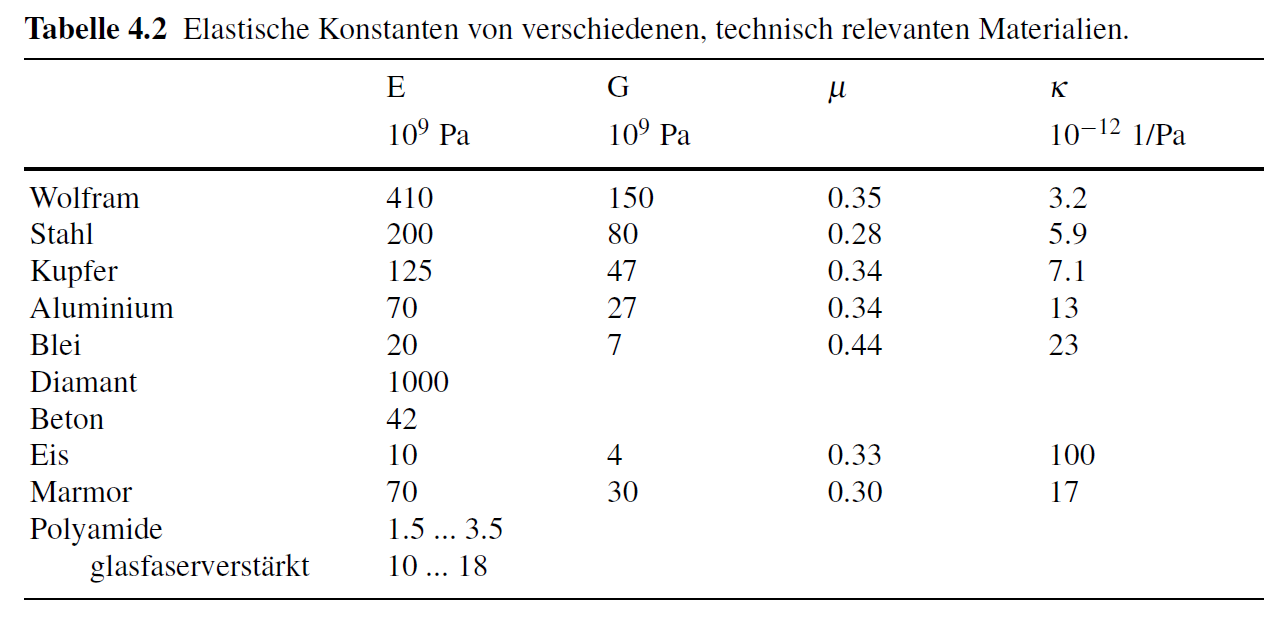
\includegraphics[height=5.5cm,keepaspectratio=true]{Images/elastische_konstanten.png}\\
	
	
	\refkuchling{674f.}, Tabelle 56, Molare Masse = $A_R$
	\begin{tabular}{ |l|c|r| }
		\hline
		Verbindung & Summeformel & Molare Masse \\
		\hline
		Luft (78\%,21\%, 1\%) & $N_2 O_2 Ar$ & $28.949$ g/mol \\
		Argon 		& $Ar$ 		& $39.948$ g/mol \\
		Methan 		& $CH_4$ 	& $16.043$ g/mol \\
		Sauerstoff 	& $O_2$ 	& $31.999$ g/mol \\
		Stickstoff	& $N_2$ 	& $28.013$ g/mol \\
		Wasser 		& $H_2 O$ 	& $18.015$ g/mol \\
		Wasserstoff & $H_2$ 	&  $2.016$ g/mol \\
		\hline
	\end{tabular}
	
\end{center}
